% Homework #6 - Pre-processing the Adult Dataset
% Build: xelatex -interaction=nonstopmode hw6_preprocess_answer.tex   (run twice)
\documentclass[11pt,a4paper]{article}

\usepackage{fontspec}
\usepackage[margin=2.2cm]{geometry}
\usepackage{booktabs}
\usepackage{tabularx}
\usepackage{longtable}
\usepackage{graphicx}
\usepackage{float}      % [H] pins tables/figures where they are written
\usepackage{adjustbox}
\usepackage{xcolor}
\usepackage{underscore}      % lets snake_case / kebab-case print literally
\usepackage{enumitem}
\usepackage{amsmath}
\usepackage{amssymb}
\usepackage[hidelinks]{hyperref}
\usepackage{titlesec}
\usepackage{caption}

\setmainfont{Latin Modern Roman}
% Latin Modern Mono ships no bold face, and column headers here are bold -> use DejaVu
% Sans Mono, which has a real bold. Scaled down to match the Roman x-height.
\setmonofont{DejaVu Sans Mono}[Scale=0.80]

\definecolor{hdr}{HTML}{1F3864}
\definecolor{acc}{HTML}{C0392B}
\definecolor{lightrow}{HTML}{F2F5FA}

\titleformat{\section}{\Large\bfseries\color{hdr}}{\thesection}{0.6em}{}
\titleformat{\subsection}{\large\bfseries\color{hdr}}{\thesubsection}{0.6em}{}
\titleformat{\subsubsection}{\bfseries}{\thesubsubsection}{0.6em}{}

\captionsetup{font=small,labelfont={bf,color=hdr}}
\setlist[itemize]{topsep=3pt,itemsep=2pt,parsep=0pt,leftmargin=1.4em}
\setlist[enumerate]{topsep=3pt,itemsep=2pt,parsep=0pt,leftmargin=1.6em}
\renewcommand{\arraystretch}{1.18}

% Verdict markers used in the decision tables.
\newcommand{\yes}{\textcolor{hdr}{$\checkmark$}}
\newcommand{\no}{\textcolor{acc}{$\times$}}
\usepackage{array}
% Ragged-right wrapping column - justification in narrow columns
% stretches word gaps badly.
\newcolumntype{L}[1]{>{\raggedright\arraybackslash}p{#1}}

\newcommand{\code}[1]{\texttt{\small #1}}

\begin{document}

% ------------------------------------------------------------------ title
\begin{center}
  {\LARGE\bfseries\color{hdr} Homework \#6 --- Pre-processing the Adult Dataset}\\[4pt]
  {\large for Predicting Socio-Economic Status (\code{income > 50K})}\\[10pt]
  {\normalsize Student ID: \textbf{6710503739}}\\[2pt]
  {\small Deliverables: \code{6710503739\_hw\#6\_preprocess.ipynb} (analysis)
   $\cdot$ this report}
\end{center}
\vspace{4pt}
\hrule
\vspace{10pt}

\noindent
\textbf{Dataset.} \code{adult.csv} --- \textbf{48{,}842} rows $\times$ \textbf{15} columns
(14 predictors + the \code{income} label). \textbf{Target balance:} 37{,}155 rows
\code{<=50K} vs 11{,}687 rows \code{>50K}, i.e.\ a \textbf{23.93\,\%} positive rate --- the
classes are imbalanced at roughly 1:3.

\medskip
\noindent
\textbf{Note on column names.} This copy of the dataset spells two columns slightly
differently from the attribute description: \code{educational-num} (description:
\emph{education-num}) and \code{gender} (description: \emph{sex}). The meaning is
identical; the file's own spelling is used throughout.

\medskip
\noindent
\textbf{Reproducibility.} Every figure and every number in this report was produced by the
accompanying notebook, which runs end-to-end without error. The notebook writes its
headline statistics to \code{report\_stats.json}, and this report quotes those values, so
the two cannot disagree.

% ================================================================== PHASE 1
\section{Phase 1 --- Exploratory Data Analysis}

\subsection{Descriptive statistics for the numerical features}

\begin{table}[H]
\centering
\caption{Summary statistics for the six numerical features. CV = std\,/\,mean, a
scale-free measure of spread.}
\small
\begin{adjustbox}{max width=\linewidth}
\begin{tabular}{lrrrrrrrr}
\toprule
\textbf{Feature} & \textbf{Mean} & \textbf{Median} & \textbf{Mode} & \textbf{Std} &
\textbf{Min} & \textbf{Max} & \textbf{Skew} & \textbf{CV} \\
\midrule
age             & 38.64      & 37.0     & 36      & 13.71      & 17 & 90        & $+0.56$ & 0.35 \\
fnlwgt          & 189{,}664  & 178{,}145& 203{,}488 & 105{,}604 & 12{,}285 & 1{,}490{,}400 & $+1.44$ & 0.56 \\
educational-num & 10.08      & 10.0     & 9       & 2.57       & 1  & 16        & $-0.32$ & 0.26 \\
capital-gain    & 1{,}079.07 & 0.0      & 0       & 7{,}452.02 & 0  & 99{,}999  & $\mathbf{+11.89}$ & \textbf{6.91} \\
capital-loss    & 87.50      & 0.0      & 0       & 403.00     & 0  & 4{,}356   & $\mathbf{+4.57}$  & \textbf{4.61} \\
hours-per-week  & 40.42      & 40.0     & 40      & 12.39      & 1  & 99        & $+0.24$ & 0.31 \\
\bottomrule
\end{tabular}
\end{adjustbox}
\end{table}

\subsubsection*{Interpretation --- which features have high variance or significant skew}

\textbf{Variance.} In raw units \code{fnlwgt} dominates everything else
(std $\approx$ 105{,}604). But \code{fnlwgt} is a \emph{survey weight} --- how many people
in the population the row represents --- not a property of the person, so its spread is an
artefact of the sampling design rather than a signal about income. Comparing raw variances
across features with different units is misleading, so the \textbf{coefficient of
variation} is the fairer measure. On that basis:

\begin{itemize}
  \item \code{capital-gain} (CV $=6.91$) and \code{capital-loss} (CV $=4.61$) are the
        genuinely extreme features --- their standard deviation is several times their own
        mean;
  \item \code{fnlwgt} is moderate (CV $=0.56$);
  \item \code{age}, \code{educational-num} and \code{hours-per-week} are tight
        (CV $=0.26$--$0.35$).
\end{itemize}

\textbf{Skew.} A symmetric feature has skew $\approx 0$; $|\text{skew}|>1$ is normally
called strong. Ranked worst first:

\begin{itemize}
  \item \code{capital-gain}, skew $\mathbf{+11.89}$ --- by far the worst in the dataset.
        91.74\,\% of rows are exactly $0$ and a thin tail runs to 99{,}999. This is a
        \emph{zero-inflated} feature, not a bell curve. Its kurtosis of 152.7 confirms an
        extremely heavy tail.
  \item \code{capital-loss}, skew $\mathbf{+4.57}$ --- the same zero-inflated shape
        (95.33\,\% zeros).
  \item \code{fnlwgt}, skew $+1.44$ --- a moderate right tail.
  \item \code{age} ($+0.56$), \code{educational-num} ($-0.32$) and \code{hours-per-week}
        ($+0.24$) are near-symmetric and need no transformation.
\end{itemize}

\noindent
The two capital features are the ones that would distort any distance- or gradient-based
model, and they are what the outlier strategy in Phase~2 addresses.

\subsection{Data-quality audit}

\subsubsection*{Data type of every column}

\begin{table}[H]
\centering
\caption{Column-by-column type audit: 6 numerical, 9 categorical (one of which is the target).}
\small
\begin{adjustbox}{max width=\linewidth}
\begin{tabular}{llrl}
\toprule
\textbf{Column} & \textbf{Kind} & \textbf{Distinct} & \textbf{Notes} \\
\midrule
age             & Numerical (continuous)  & 74 & years, 17--90 \\
workclass       & Categorical (nominal)   & 9  & includes the \code{?} sentinel \\
fnlwgt          & Numerical (continuous)  & 28{,}523 & survey weight, not a personal attribute \\
education       & Categorical (ordinal)   & 16 & duplicate of \code{educational-num} (see \S1.3.2) \\
educational-num & Numerical (ordinal)     & 16 & rank code 1--16 \\
marital-status  & Categorical (nominal)   & 7  & \\
occupation      & Categorical (nominal)   & 15 & includes the \code{?} sentinel \\
relationship    & Categorical (nominal)   & 6  & \\
race            & Categorical (nominal)   & 5  & \\
gender          & Categorical (binary)    & 2  & Male / Female \\
capital-gain    & Numerical (continuous)  & 123 & zero-inflated, top-coded at 99{,}999 \\
capital-loss    & Numerical (continuous)  & 99 & zero-inflated \\
hours-per-week  & Numerical (continuous)  & 96 & \\
native-country  & Categorical (nominal)   & 42 & includes the \code{?} sentinel \\
income          & Categorical (target)    & 2  & \code{<=50K} / \code{>50K} \\
\bottomrule
\end{tabular}
\end{adjustbox}
\end{table}

\noindent
\code{educational-num} is listed as \emph{ordinal} rather than plain numerical because the
distinction matters downstream: an ordinal code must keep its ranking and must \emph{not}
be one-hot encoded like a nominal column.

\subsubsection*{Missing values --- the \code{?} sentinel}

\code{pandas} reports \textbf{zero} \code{NaN} in this file. That is misleading: in the
Adult dataset an unknown value is stored as the literal character \textbf{\code{?}}, which
\code{read\_csv} loads as an ordinary string. The audit therefore searched every text
column for the sentinel explicitly.

\begin{table}[H]
\centering
\caption{Missing values found by searching for the \code{?} sentinel. All other columns: 0.}
\small
\begin{tabular}{lrr}
\toprule
\textbf{Column} & \textbf{\# missing} & \textbf{\% of rows} \\
\midrule
occupation      & 2{,}809 & 5.75\,\% \\
workclass       & 2{,}799 & 5.73\,\% \\
native-country  & 857     & 1.75\,\% \\
\midrule
\textbf{Rows with at least one \code{?}} & \textbf{3{,}620} & \textbf{7.41\,\%} \\
\bottomrule
\end{tabular}
\end{table}

\noindent
\textbf{The missingness is not random.} \code{occupation} and \code{workclass} are missing
on almost exactly the same rows: \textbf{2{,}799 of the 2{,}809} \code{occupation} gaps
coincide with a missing \code{workclass}. The 10 rows where \code{occupation} is missing
but \code{workclass} is present are \emph{all} \code{Never-worked} --- for those people an
occupation genuinely does not exist. So ``missing'' here largely encodes
\emph{``not currently in the labour force''} (retired, unemployed, never worked), which is a
structurally meaningful fact rather than a lost measurement. \code{native-country} is a
different case: a small, scattered set of unrecorded values. This distinction drives the
imputation decision in \S3.1.

\medskip
\noindent
\textbf{Duplicates.} 52 rows are exact duplicates of another row (0.11\,\%).

\subsection{Categorical analysis}

\subsubsection*{Distinct labels present in each categorical column}

\begin{table}[H]
\centering
\caption{Every distinct label found in each categorical column, as it appears in the file.}
\small
\begin{adjustbox}{max width=\linewidth}
\begin{tabular}{L{2.6cm}rL{11.2cm}}
\toprule
\textbf{Column} & \textbf{\#} & \textbf{Labels} \\
\midrule
workclass & 9 &
\code{?}, Federal-gov, Local-gov, Never-worked, Private, Self-emp-inc, Self-emp-not-inc,
State-gov, Without-pay \\
education & 16 &
10th, 11th, 12th, 1st-4th, 5th-6th, 7th-8th, 9th, Assoc-acdm, Assoc-voc, Bachelors,
Doctorate, HS-grad, Masters, Preschool, Prof-school, Some-college \\
marital-status & 7 &
Divorced, Married-AF-spouse, Married-civ-spouse, Married-spouse-absent, Never-married,
Separated, Widowed \\
occupation & 15 &
\code{?}, Adm-clerical, Armed-Forces, Craft-repair, Exec-managerial, Farming-fishing,
Handlers-cleaners, Machine-op-inspct, Other-service, Priv-house-serv, Prof-specialty,
Protective-serv, Sales, Tech-support, Transport-moving \\
relationship & 6 &
Husband, Not-in-family, Other-relative, Own-child, Unmarried, Wife \\
race & 5 &
Amer-Indian-Eskimo, Asian-Pac-Islander, Black, Other, White \\
gender & 2 & Female, Male \\
native-country & 42 &
\code{?}, Cambodia, Canada, China, Columbia, Cuba, Dominican-Republic, Ecuador,
El-Salvador, England, France, Germany, Greece, Guatemala, Haiti,
Holand-Netherlands, Honduras, Hong, Hungary, India, Iran, Ireland, Italy, Jamaica,
Japan, Laos, Mexico, Nicaragua, Outlying-US(Guam-USVI-etc), Peru, Philippines, Poland,
Portugal, Puerto-Rico, Scotland, South, Taiwan, Thailand, Trinadad\&Tobago,
United-States, Vietnam, Yugoslavia \\
income (target) & 2 & \code{<=50K}, \code{>50K} \\
\bottomrule
\end{tabular}
\end{adjustbox}
\end{table}

\noindent
Note that \code{?} appears in the label list of exactly the three columns identified above
--- confirming the sentinel is being read as a legitimate category and must be handled
before encoding. \code{native-country} is heavily concentrated: \textbf{91.4\,\%} of the
known values are \code{United-States}, and most of the remaining 40 countries hold well
under 1\,\% each.

\subsubsection*{\code{education} vs \code{educational-num} --- why keeping both is redundant}

Grouping the data by \code{education} shows that each of the 16 text labels maps to
\textbf{exactly one} \code{educational-num} value, and each of the 16 numeric values maps
back to exactly one label --- a verified \textbf{perfect one-to-one mapping}:

\begin{center}
\small
\code{Preschool}$\to$1, \code{1st-4th}$\to$2, \code{5th-6th}$\to$3, \code{7th-8th}$\to$4,
\code{9th}$\to$5, \code{10th}$\to$6, \code{11th}$\to$7, \code{12th}$\to$8,
\code{HS-grad}$\to$9, \code{Some-college}$\to$10, \code{Assoc-voc}$\to$11,
\code{Assoc-acdm}$\to$12, \code{Bachelors}$\to$13, \code{Masters}$\to$14,
\code{Prof-school}$\to$15, \code{Doctorate}$\to$16
\end{center}

\noindent
The two columns therefore carry \emph{exactly} the same information --- one variable
expressed twice, once as text and once as an integer code. Keeping both is redundant and
actively harmful:

\begin{enumerate}
  \item \textbf{Perfect multicollinearity.} A model given both sees two features related
        deterministically. For linear models the coefficients become unidentifiable (the
        design matrix is rank-deficient); for tree ensembles the importance of ``education''
        is split arbitrarily between two identical columns, so neither looks important.
  \item \textbf{Wasted dimensionality.} One-hot encoding \code{education} would add 16
        sparse columns that duplicate a single existing integer column.
  \item \textbf{Loss of order.} \code{educational-num} already encodes the \emph{rank}
        (a Doctorate outranks a Bachelors). One-hot encoding the text version discards that
        ordering entirely.
\end{enumerate}

\noindent
\textbf{Decision:} drop \code{education}, keep \code{educational-num}, which is already a
correct ordinal encoding. \S3.2 proves this by re-deriving the ordinal code from scratch
with an explicitly stated rank order and confirming it reproduces \code{educational-num}
value-for-value.

% ================================================================== PHASE 2
\section{Phase 2 --- Visual Discovery \& Outlier Handling}

\subsection{Distributions of \code{age}, \code{hours-per-week} and \code{capital-gain}}

\begin{figure}[H]
\centering
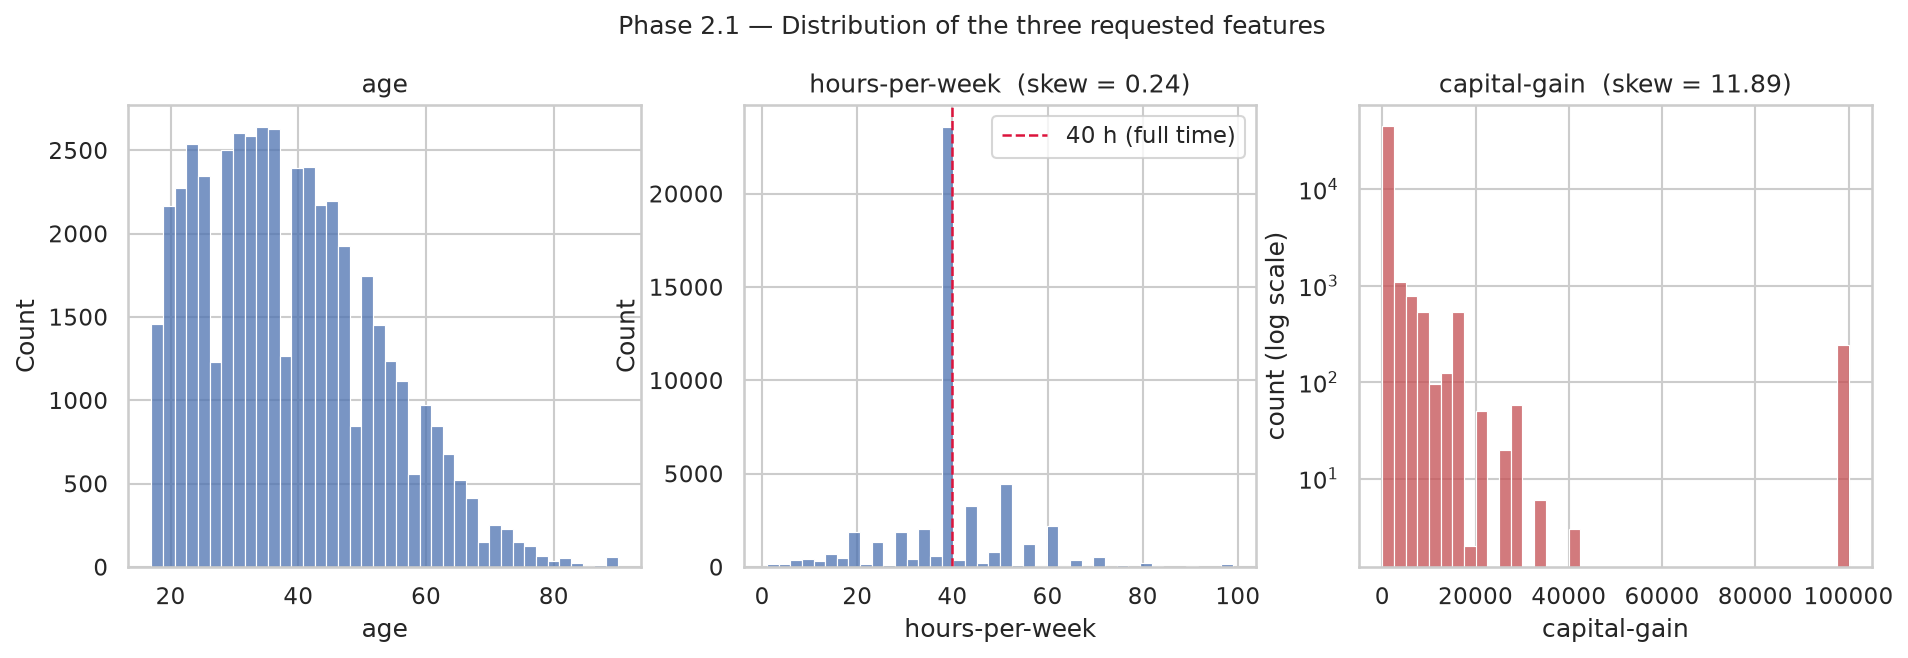
\includegraphics[width=\linewidth]{figures/hist_three.png}
\caption{Histograms of the three requested features. \code{capital-gain} uses a
logarithmic count axis --- on a linear axis only the zero bar is visible.}
\end{figure}

\begin{itemize}
  \item \textbf{\code{age}} --- right-skewed but entirely plausible: a peak in the late
        twenties to thirties, a long thin tail into old age, hard-stopped at exactly 90.
  \item \textbf{\code{hours-per-week}} --- a huge spike at exactly 40 (the standard working
        week), with smaller spikes at 20, 45, 50 and 60. This is not a smooth distribution
        but a mixture of socially conventional values, which is why its interquartile range
        is only 5 hours.
  \item \textbf{\code{capital-gain}} --- visually a single bar at zero. On the log-count
        axis the tail appears, and a \textbf{separate isolated bar sits exactly at
        99{,}999}, clearly detached from the rest of the distribution.
\end{itemize}

\begin{figure}[H]
\centering
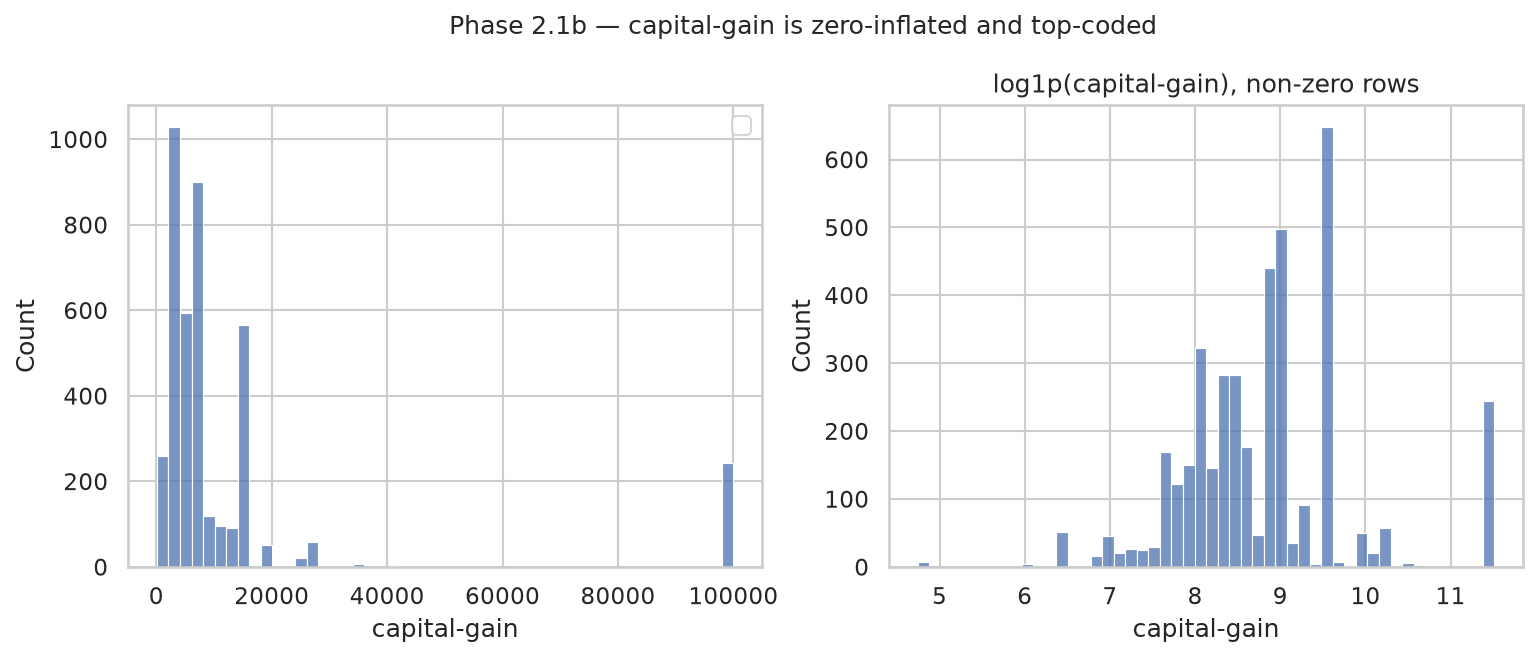
\includegraphics[width=0.92\linewidth]{figures/hist_capgain_zoom.png}
\caption{\code{capital-gain} restricted to its 4{,}035 non-zero rows. Left: the raw values,
with the 99{,}999 ceiling marked. Right: the same values after \code{log1p}.}
\end{figure}

\noindent
Zooming in confirms it: the largest value \emph{below} the ceiling is \textbf{41{,}310}, and
then \textbf{244 rows} sit on exactly \textbf{99{,}999} with nothing in between. No natural
distribution produces a cluster on a single round ceiling --- this is census
\textbf{top-coding}: every gain above the cut-off was clipped to 99{,}999.

\subsection{Box plots and IQR outlier counts}

\begin{figure}[H]
\centering
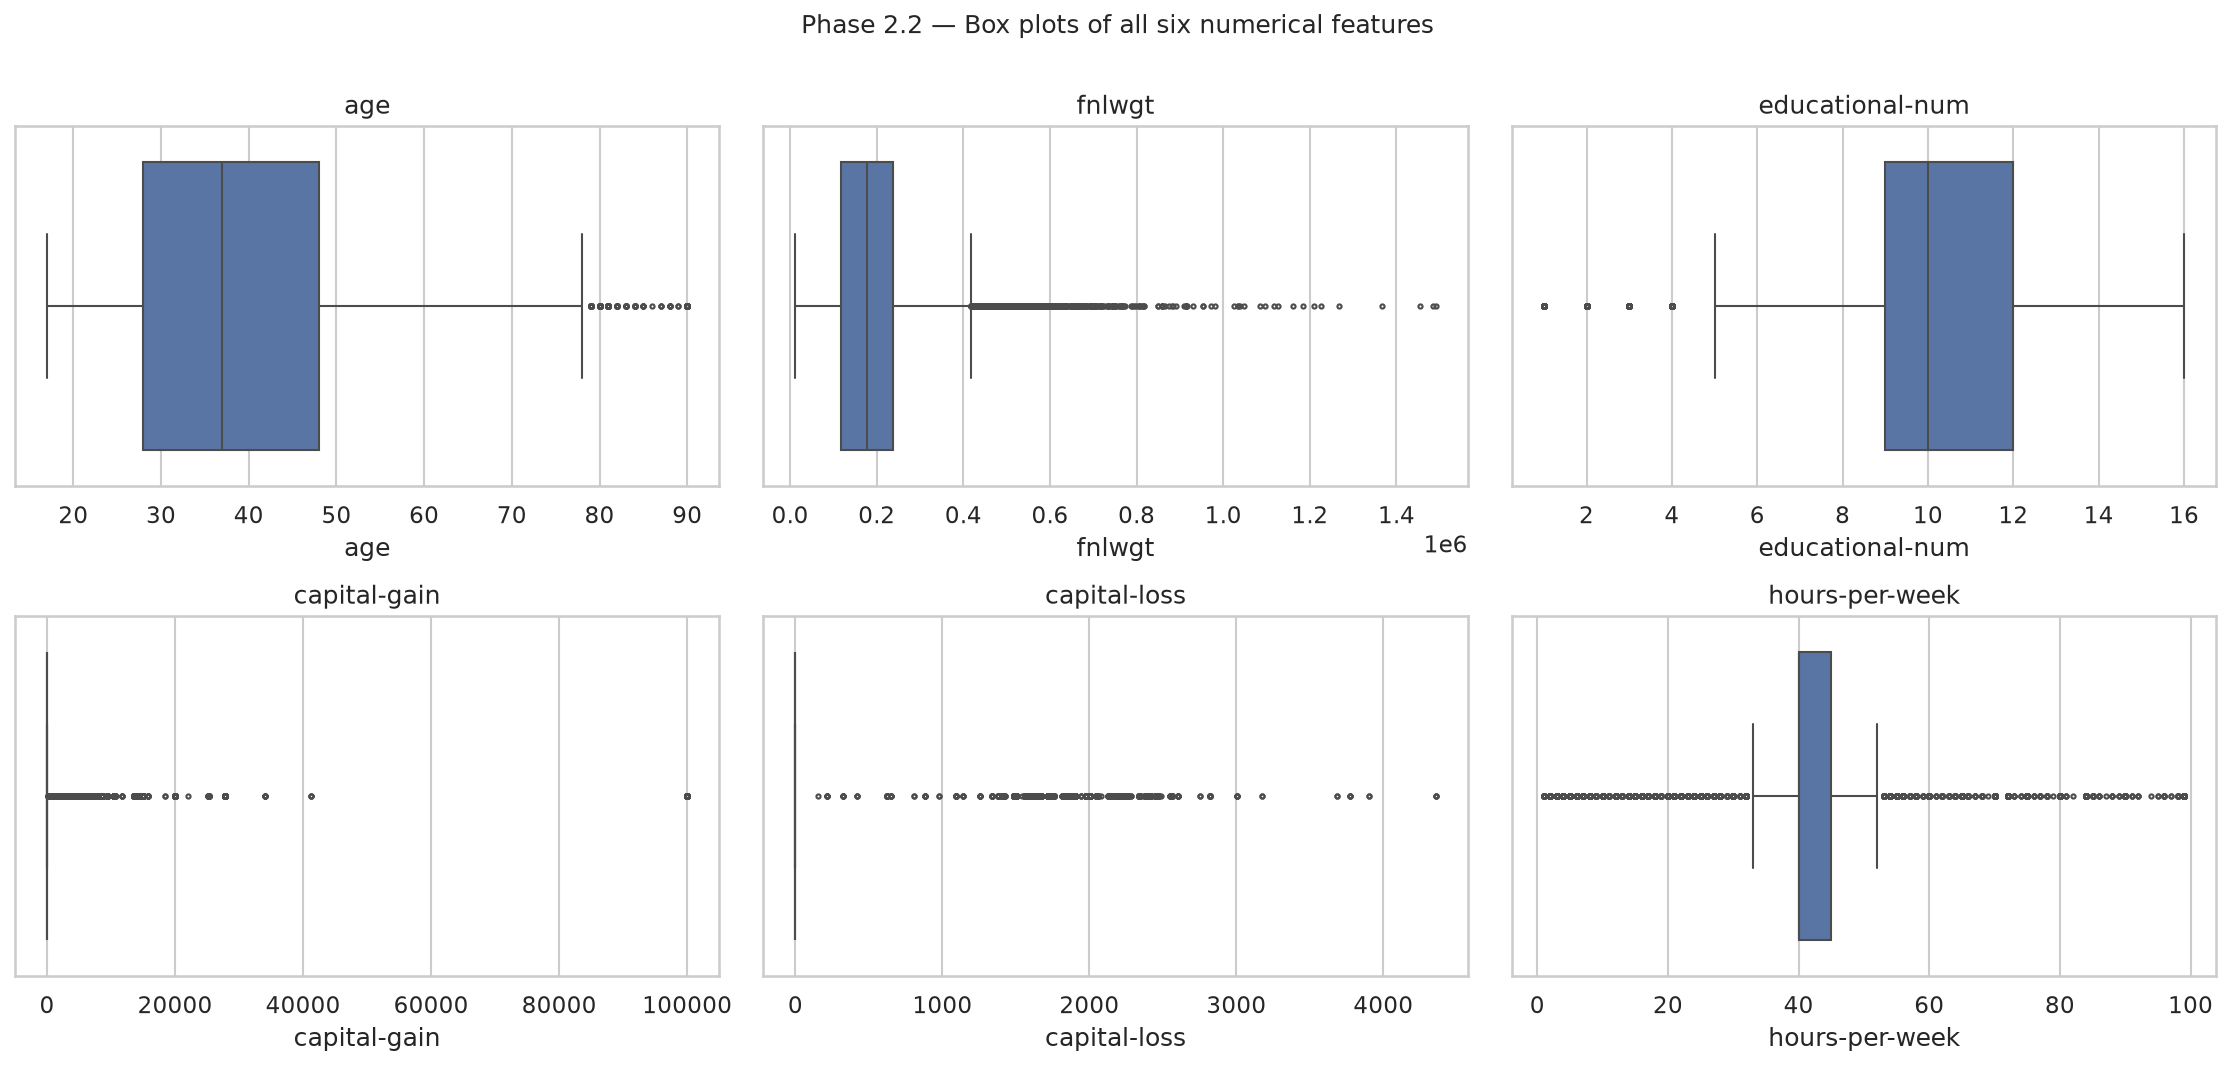
\includegraphics[width=\linewidth]{figures/boxplots.png}
\caption{Box plots of all six numerical features on their raw scales.}
\end{figure}

\begin{table}[H]
\centering
\caption{Outliers by the standard $1.5\times$IQR rule. Note that for \code{capital-gain}
and \code{capital-loss} the IQR is \emph{zero} (Q1 = Q3 = 0), so the rule flags
\emph{every} non-zero value as an outlier.}
\small
\begin{tabular}{lrrrrrr}
\toprule
\textbf{Feature} & \textbf{Q1} & \textbf{Q3} & \textbf{IQR} &
\textbf{Lower fence} & \textbf{Upper fence} & \textbf{\# (\%) flagged} \\
\midrule
age             & 28.0      & 48.0      & 20.0      & $-2.0$       & 78.0       & 216 (0.44\,\%) \\
fnlwgt          & 117{,}551 & 237{,}642 & 120{,}092 & $-62{,}587$  & 417{,}779  & 1{,}453 (2.97\,\%) \\
educational-num & 9.0       & 12.0      & 3.0       & 4.5          & 16.5       & 1{,}794 (3.67\,\%) \\
capital-gain    & 0.0       & 0.0       & 0.0       & 0.0          & 0.0        & 4{,}035 (8.26\,\%) \\
capital-loss    & 0.0       & 0.0       & 0.0       & 0.0          & 0.0        & 2{,}282 (4.67\,\%) \\
hours-per-week  & 40.0      & 45.0      & 5.0       & 32.5         & 52.5       & 13{,}496 (27.63\,\%) \\
\bottomrule
\end{tabular}
\end{table}

\subsection{Outlier strategy}

\textbf{Feature chosen: \code{capital-gain}} --- the most extreme feature in the dataset
(skew $+11.89$, maximum 99{,}999, every non-zero value flagged by the IQR rule).
\code{age} is discussed as a secondary case.

\subsubsection*{Are these errors or real-world extremes?}

Both --- in different ways, and the evidence separates them cleanly:

\begin{table}[H]
\centering
\small
\begin{adjustbox}{max width=\linewidth}
\begin{tabular}{L{7.4cm}L{8.4cm}}
\toprule
\textbf{Observation} & \textbf{Reading} \\
\midrule
91.74\,\% of rows are exactly 0 &
\textbf{Real.} Most people realise no capital gain in a year. Zero is a true value, not a
gap --- so this is not a missing-data problem. \\
A smooth tail from a few hundred up to 41{,}310 &
\textbf{Real-world extremes.} Genuine investment income. These people really do earn more,
and the values behave like a continuous distribution. \\
Exactly 244 rows at exactly 99{,}999, with a gap of $\approx$\,58{,}000 below them &
\textbf{An artefact.} Census \textbf{top-coding} --- everything above the cut-off was
clipped to one value. 99{,}999 is a censoring flag, not a measurement. \\
\bottomrule
\end{tabular}
\end{adjustbox}
\end{table}

\noindent
Before deciding, the notebook checked whether the tail is actually informative:

\begin{table}[H]
\centering
\caption{\code{>50K} rate by \code{capital-gain} band.}
\small
\begin{tabular}{lrr}
\toprule
\textbf{capital-gain band} & \textbf{\# rows} & \textbf{\% earning \code{>50K}} \\
\midrule
0                    & 44{,}807 & 20.5\,\% \\
1--5{,}000           & 1{,}584  & 17.9\,\% \\
5{,}000--20{,}000    & 2{,}070  & 88.7\,\% \\
20{,}000--99{,}998   & 137      & 92.7\,\% \\
99{,}999 (top-coded) & 244      & \textbf{100.0\,\%} \\
\bottomrule
\end{tabular}
\end{table}

\noindent
The relationship is \emph{not} monotonic at the bottom --- the rate dips slightly from
20.5\,\% at zero to 17.9\,\% for small gains (small gains come mostly from modest earners)
--- but above 5{,}000 it jumps to 88.7\,\%, then 92.7\,\%, and reaches \textbf{100\,\%} for
the top-coded group. The tail is therefore among the strongest predictors in the dataset,
and the top-coded rows are not junk to be discarded: they are the richest people in the
sample.

\subsubsection*{Decision: \textbf{KEEP} the outliers, but transform them}

\begin{table}[H]
\centering
\small
\begin{adjustbox}{max width=\linewidth}
\begin{tabular}{L{3.8cm}L{12.0cm}}
\toprule
\textbf{Option} & \textbf{Verdict} \\
\midrule
\textbf{Remove} the rows &
\no~\textbf{Rejected.} The $1.5\times$IQR rule flags 8.26\,\% of rows on
\code{capital-gain} alone, and \textbf{41.53\,\% of the entire dataset (20{,}284 rows)}
once every numerical column is considered --- \code{hours-per-week} alone flags 27.63\,\%,
because its IQR is a mere 5 hours. Worse, removal would delete almost every high earner,
i.e.\ exactly the signal the model is being built to detect, biasing the target
distribution. \\
\textbf{Replace} (winsorise, or impute with the median) &
\no~\textbf{Rejected as the primary treatment.} These are not measurement errors.
Replacing 99{,}999 with the median would destroy the single strongest predictor in the
dataset (a group with a 100\,\% \code{>50K} rate). \\
\textbf{Keep}, but reshape the scale &
\yes~\textbf{Chosen.} Retains every row and every ordering, while removing the numerical
dominance that the raw scale would give the feature. \\
\bottomrule
\end{tabular}
\end{adjustbox}
\end{table}

\noindent
Concretely, this decision is implemented in Phases 3--4 as:

\begin{enumerate}
  \item \textbf{Keep every row.} No row is deleted for being an outlier. (The 52 exact
        duplicates \emph{are} dropped --- but as a data-collection artefact, not as
        outliers.)
  \item \textbf{Apply \code{log1p}} to \code{capital-gain} and \code{capital-loss}. This
        compresses the skew towards symmetry so the feature can no longer dominate a
        distance metric, while preserving the \emph{order} of every value. \code{log1p}
        rather than \code{log} because it maps the 91.74\,\% of exact zeros to 0 instead of
        $-\infty$.
  \item \textbf{Add an explicit \code{capital-gain-topcoded} flag} for the 244 censored
        rows, so a model can learn ``this value is a ceiling, not a measurement'' rather
        than treating 99{,}999 as a precise amount.
\end{enumerate}

\noindent
\textbf{\code{age} is treated differently and more simply.} The IQR rule flags 216 people
over 78, but a 90-year-old is a perfectly real survey respondent, so those rows are
\textbf{kept untransformed}. The pile-up at exactly 90 is the same top-coding artefact
(age was capped at 90), but with a negligible effect on the feature's scale, so no
transform is warranted.

% ================================================================== PHASE 3
\section{Phase 3 --- Data Pre-processing \& Transformation}

\subsection{Handling missing values}

\textbf{Step 1 --- make the missingness visible.} All text columns are whitespace-stripped
and the \code{?} sentinel is replaced with a real \code{NaN}, so that standard pandas
missing-value tooling works at all.

\begin{figure}[H]
\centering
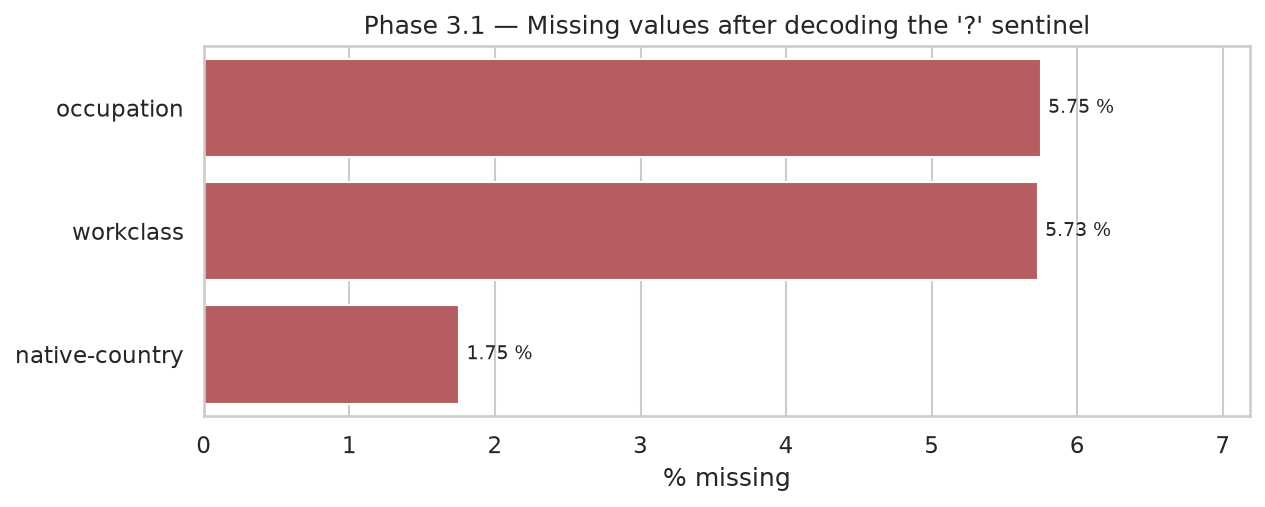
\includegraphics[width=0.78\linewidth]{figures/missing_bar.png}
\caption{Missing values once the \code{?} sentinel has been decoded to \code{NaN}.}
\end{figure}

\noindent
\textbf{Step 2 --- choose the strategy.} The audit in \S1.2 showed these gaps are not one
homogeneous problem, so a single blanket rule would be wrong. \textbf{Two different
strategies} are applied.

\subsubsection*{(a) \code{workclass} and \code{occupation} $\to$ a new explicit category \code{"Unknown"}}

\textbf{Why.} These two columns are missing on the same 2{,}799 rows, and the pattern is
structural: these are people outside the labour force. ``No workclass'' is a \emph{fact
about the person}, not a lost value. The two groups are demonstrably different populations:

\begin{table}[H]
\centering
\small
\begin{tabular}{lrrrr}
\toprule
& \textbf{\# rows} & \textbf{Mean age} & \textbf{Mean hours/week} & \textbf{\% \code{>50K}} \\
\midrule
\code{workclass} missing & 2{,}795  & 40.2 & 31.8 & \textbf{9.5\,\%} \\
\code{workclass} present & 45{,}995 & 38.6 & 41.0 & \textbf{24.8\,\%} \\
\bottomrule
\end{tabular}
\end{table}

\noindent
The missing group is older, works roughly nine fewer hours a week, and is about
\textbf{2.6 times less likely} to earn \code{>50K}. Imputing with the mode
(\code{Private} / \code{Prof-specialty}) would \emph{fabricate a job for 2{,}795 retired or
unemployed people} and erase a genuinely predictive signal. Encoding the gap as its own
\code{"Unknown"} category keeps that signal available to the model and --- since these
columns are about to be one-hot encoded anyway --- costs only one extra binary column each.

\subsubsection*{(b) \code{native-country} $\to$ mode imputation (\code{United-States})}

\textbf{Why.} Only 1.75\,\% of rows are affected, there is no structural story behind the
gap (an unrecorded country is simply an unrecorded field, not a statement about the
person), and the column is overwhelmingly dominated by one value --- \textbf{91.4\,\%} of
all \emph{known} countries are \code{United-States}. Mode imputation on a 1.75\,\% gap in a
91\,\%-dominant column shifts the column's distribution by well under two percentage
points, and avoids inflating the one-hot matrix with a 42nd category that would carry
almost no information.

\medskip
\noindent
After imputation the dataset contains \textbf{zero} missing values (asserted in the
notebook).

\subsection{Dropping the redundant column --- with proof}

Before dropping \code{education}, the ordinal encoding was rebuilt from scratch using
scikit-learn's \code{OrdinalEncoder} with the academic rank order stated explicitly
(\code{Preschool} $<$ \code{1st-4th} $<\dots<$ \code{Prof-school} $<$ \code{Doctorate}).
The hand-built code reproduces \code{educational-num} exactly --- \textbf{value for value,
across all 48{,}790 rows} --- which confirms the redundancy claim of \S1.3.2 empirically
rather than by assertion. \code{education} is then dropped.

\subsection{Categorical encoding}

Three different encodings are used, because these are three different kinds of variable.
Using one-hot everywhere would throw away a real ordering; using label encoding everywhere
would invent an ordering that does not exist.

\begin{table}[H]
\centering
\small
\begin{adjustbox}{max width=\linewidth}
\begin{tabular}{L{2.3cm}L{5.2cm}L{2.9cm}L{5.4cm}}
\toprule
\textbf{Kind} & \textbf{Columns} & \textbf{Encoding} & \textbf{Reason} \\
\midrule
\textbf{Ordinal} &
\code{educational-num} &
already a 1--16 rank code &
The ranking is real and meaningful (a Doctorate outranks a Bachelors), so preserve it. \\
\textbf{Binary} &
\code{gender}, \code{income} (target) &
label encode 0/1 &
With two levels, one-hot and label encoding are mathematically equivalent; 0/1 is simpler
and adds no columns. \code{Male}=1, \code{>50K}=1. \\
\textbf{Nominal} &
\code{workclass}, \code{marital-status}, \code{occupation}, \code{relationship},
\code{race}, \code{native-country} &
one-hot, \mbox{\code{drop\_first=True}} &
There is no sensible ordering between e.g.\ \code{Sales} and \code{Tech-support}; a label
code would make a model believe one is ``greater than'' the other. \\
\bottomrule
\end{tabular}
\end{adjustbox}
\end{table}

\noindent
An extra engineered column, \code{capital-gain-topcoded}, is added here per the Phase~2
decision.

\medskip
\noindent
\textbf{Why \code{drop\_first=True}.} With $k$ levels only $k-1$ indicator columns are
needed --- the dropped reference level is implied when all the others are 0. Keeping all
$k$ creates the \emph{dummy-variable trap}: the columns sum to 1 for every row, so the
design matrix is rank-deficient and linear-model coefficients become unidentifiable. This
also removes 6 redundant columns.

\medskip
\noindent
\textbf{Result:} \textbf{15 columns $\to$ 86 columns} (48{,}790 rows), all numeric.

% ================================================================== PHASE 4
\section{Phase 4 --- Scaling \& Final Preparation}

\subsection{The skew transform (applied before scaling)}

Scaling does \emph{not} fix skew --- standardising \code{capital-gain} would leave a
feature with skew 11.89, merely re-centred. The \code{log1p} transform decided in \S2.3 is
therefore applied first:

\begin{table}[H]
\centering
\small
\begin{tabular}{lrr}
\toprule
\textbf{Feature} & \textbf{Skew before \code{log1p}} & \textbf{Skew after \code{log1p}} \\
\midrule
capital-gain & $+11.89$ & $\mathbf{+3.11}$ \\
capital-loss & $+4.57$  & $+4.30$ \\
\bottomrule
\end{tabular}
\end{table}

\noindent
\textbf{Reported honestly:} \code{capital-gain} improves dramatically --- skew
$11.89 \to 3.11$, and its range collapses from $0$--$99{,}999$ to $0$--$11.5$, so it can no
longer dominate a distance metric. \code{capital-loss} barely moves ($4.57 \to 4.30$), and
that is expected: 95.33\,\% of its values are exactly 0, so the residual skew comes from
the \emph{zero-inflation itself}, not from the scale of the non-zero tail --- and no
monotone transform can remove a point mass at zero. The residual skew is accepted here;
if a later model proved sensitive to it, the next step would be to split the column into a
binary \code{has-capital-loss} indicator plus the log amount.

\subsection{Train/test split \emph{before} fitting the scaler}

The data is split 80/20, stratified on \code{income}, \emph{before} the scaler is fitted:
\textbf{39{,}032 training} rows and \textbf{9{,}758 test} rows, each retaining the 23.9\,\%
\code{>50K} rate. The scaler is then fitted on the training set only and merely
\emph{applied} to the test set. Fitting it on the full dataset would leak the test set's
mean and standard deviation into training and produce an optimistically biased estimate of
model performance later.

\subsection{Feature scaling}

\textbf{Standardisation} (\code{StandardScaler}, $z = (x-\mu)/\sigma$) is chosen as the
primary method:

\begin{itemize}
  \item it does not depend on the minimum and maximum, so a single extreme value cannot
        squash every other observation into a narrow band --- which matters here precisely
        because Phase~2 decided to \emph{keep} the extremes;
  \item it is the assumption behind regularised linear models, SVMs and PCA;
  \item the 79 binary columns (77 one-hot indicators, plus \code{gender} and
        \code{capital-gain-topcoded}) are deliberately \textbf{left untouched} --- they are
        already on a 0/1 scale, and standardising them would destroy their sparsity and
        their interpretability. Only the six genuinely continuous columns are scaled.
\end{itemize}

\begin{figure}[H]
\centering
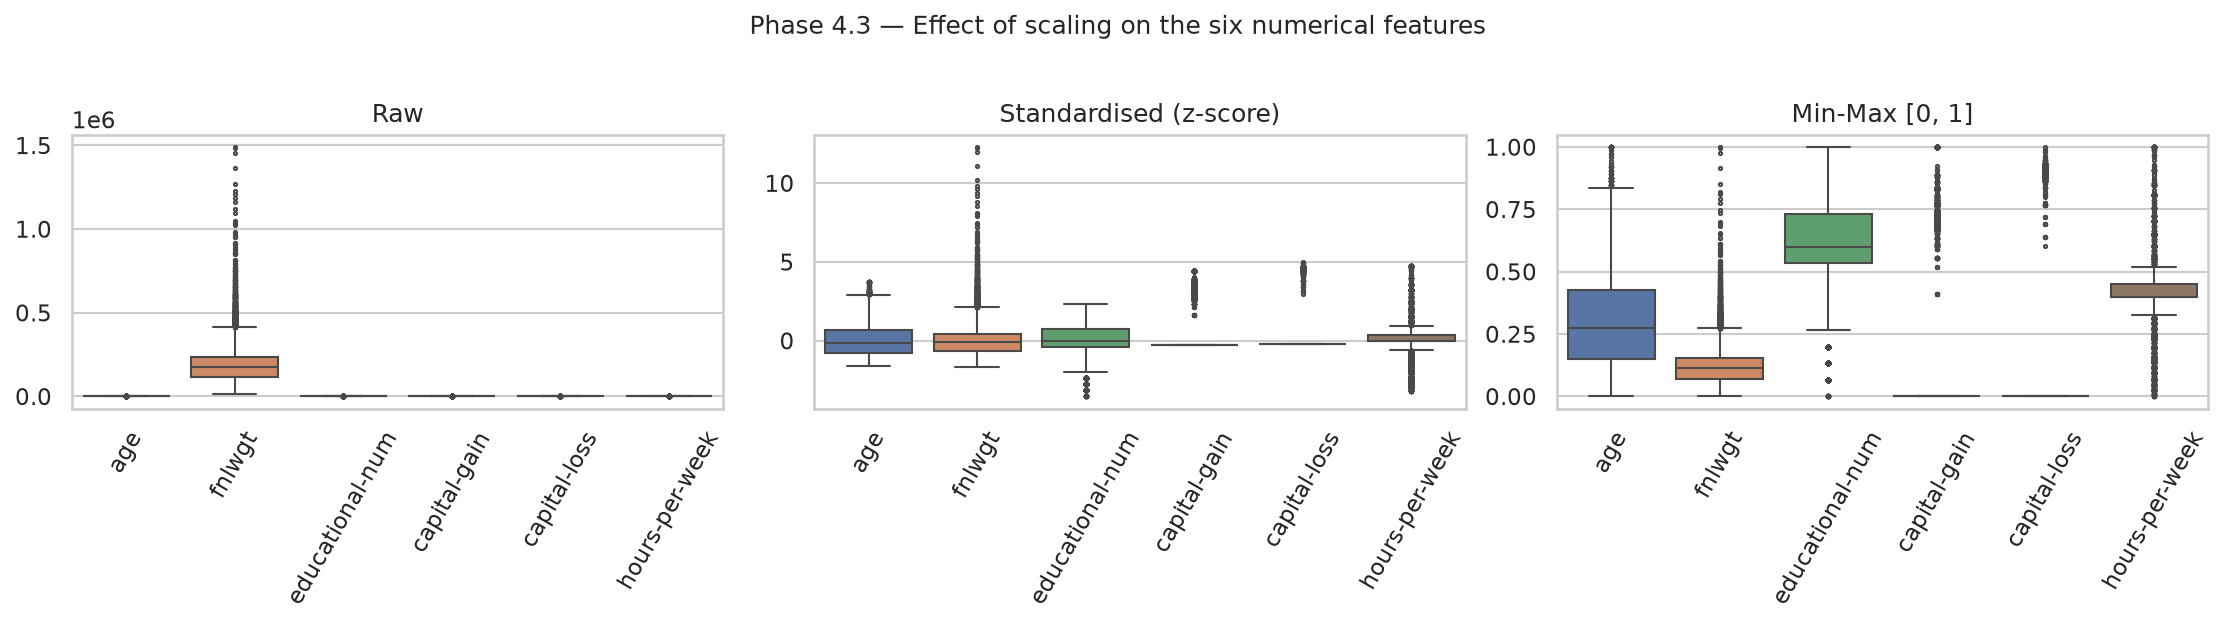
\includegraphics[width=\linewidth]{figures/scaling_compare.png}
\caption{The six numerical features before scaling, after standardisation, and after
Min-Max scaling (training set).}
\end{figure}

\noindent
The left panel shows the problem: on the raw axis \code{fnlwgt} (tens of thousands) is the
only feature visible at all --- \code{age}, \code{educational-num} and
\code{hours-per-week} are flattened to a line near zero. A distance-based model would be
deciding almost entirely on \code{fnlwgt}, which as noted in \S1.1 is a survey weight
carrying no information about the person.

\medskip
\noindent
Both scalers fix that, but the instructive difference is \textbf{\code{fnlwgt}}: its maximum
(1{,}490{,}400) is roughly six times its own Q3, so Min-Max --- which anchors on that single
most extreme value --- squeezes its entire interquartile range into about the 0.07--0.15
band, whereas standardisation leaves a box of normal size. That sensitivity to one extreme
value is exactly why standardisation was selected for the final output.

\medskip
\noindent
(\code{capital-gain} and \code{capital-loss} appear as flat lines in \emph{both} scaled
panels. That is not a scaling failure but the zero-inflation of \S2.3 showing through: with
92\,\%/95\,\% of values identical, Q1 = median = Q3, so the box has no width at any scale.)

\subsection{Final verification and output}

All six automated checks in the notebook pass:

\begin{center}
\small
\begin{tabular}{ll}
\yes~no missing values remain & \yes~target is strictly 0/1 \\
\yes~all 86 columns are numeric & \yes~scaled means $= 0$ (to $10^{-9}$) \\
\yes~no duplicate rows & \yes~scaled standard deviations $= 1$ (to $10^{-9}$) \\
\end{tabular}
\end{center}

\noindent
Files written by the notebook: \code{adult\_train\_preprocessed.csv} (39{,}032 rows),
\code{adult\_test\_preprocessed.csv} (9{,}758 rows), and
\code{adult\_encoded\_unscaled.csv} (48{,}790 rows, encoded but unscaled, for models such
as tree ensembles that do not need scaling).

% ================================================================== SUMMARY
\section{Summary of the pipeline}

\begin{table}[H]
\centering
\small
\begin{adjustbox}{max width=\linewidth}
\begin{tabular}{rL{3.5cm}L{4.6cm}L{6.6cm}}
\toprule
\textbf{\#} & \textbf{Step} & \textbf{Decision} & \textbf{Why} \\
\midrule
1  & Load & 48{,}842 $\times$ 15 & --- \\
2  & Duplicates & dropped 52 exact duplicates & identical records are a collection
     artefact, not information \\
3  & Missing \code{?} & decoded to \code{NaN} & pandas reports 0 \code{NaN} otherwise \\
4  & \code{workclass}, \code{occupation} & $\to$ \code{"Unknown"} category & the gap is
     structural (outside the labour force) and is itself predictive \\
5  & \code{native-country} & $\to$ mode \code{United-States} & 1.75\,\% gap, no structural
     story, 91.4\,\%-dominant column \\
6  & \code{education} & dropped & verified one-to-one duplicate of
     \code{educational-num} \\
7  & Outliers & \textbf{kept}, not removed & real-world extremes carrying the strongest
     income signal; removal would cost 41.5\,\% of rows \\
8  & \code{capital-gain} $=$ 99999 & flagged with a new binary column & top-coding
     artefact, not a measurement \\
9  & \code{capital-gain/loss} & \code{log1p} & skew $11.89\to3.11$ while preserving order
     (\code{capital-loss} stays skewed --- zero-inflation, not scale) \\
10 & \code{gender}, \code{income} & label encode 0/1 & binary \\
11 & 6 nominal columns & one-hot, \mbox{\code{drop\_first=True}} & no natural order; avoids the
     dummy-variable trap \\
12 & Split & 80/20 stratified, \emph{before} scaling & prevents test-set leakage into the
     scaler \\
13 & 6 continuous columns & \code{StandardScaler} & robust to the retained extremes;
     dummies left as 0/1 \\
\bottomrule
\end{tabular}
\end{adjustbox}
\end{table}

\noindent
\textbf{Outcome.} The raw 48{,}842\,$\times$\,15 table with a hidden \code{?} sentinel, a
duplicated column, an 11.9-skew feature and nine text columns has become a
\textbf{48{,}790\,$\times$\,86 fully numerical, gap-free, comparably scaled matrix}, split
into stratified train and test sets and ready for a classification model.

\end{document}
